%!TEX root = ../main.tex
\section{Data}
\subsection{Factor return series}
Factor return series are downloaded from Ken French's data library.\footnote{\url{http://mba.tuck.dartmouth.edu/pages/faculty/ken.french/data_library.html}} We download the daily Fama-French five-factor data set and merge this with the daily momentum data set. Both are available since 1963-07-01, making 1963-07-05 the first week of data. We convert each of the return series into weekly log returns for further use. 

The Mkt-RF factor is long the value-weighted return of CRSP firms on NYSE, AMEX or NASDAQ with CRSP share codes 10 or 11 and short the one-month Treasury bill rate. The remaining return series are based on zero-cost portfolios that are long certain equities and short other equities, according to a 2 x 3 sort: First, firms are sorted into one of two size groups, small and big, depending on whether the market cap is above or below the median. For each the small and big firm groups, each factor then sorts into one of three groups depending on whether the variable of interest falls below the 30\textsuperscript{th} percentile, between the 30\textsuperscript{th} and the 70\textsuperscript{th} or above the 70\textsuperscript{th}. For the five-factor data set, the factors are:
\begin{itemize}
  \item High-minus-low, is long firms above the 70\textsuperscript{th} percentile B/M (high) and short stocks below the 30\textsuperscript{th} percentile, in the small and big firm group respectively. \\
  $HML = 1/2 \cdot (Small\,value + Big\,value) - 1/2 \cdot (Small\,growth + Big\,growth)$
  \item Small-minus-big, is long firms below the 50\textsuperscript{th} percentile market cap and short firms above the 50\textsuperscript{th} percentile, in each of three groups. \\
  $SMB = 1/3 \cdot (SMB_{HML} + SMB_{RMW} + SMB_{CMA}$)
  \item Robust-minus-weak, is long firms above the 70\textsuperscript{th} percentile operating profitability and short firms below the 30\textsuperscript{th} percentile. \\
  $RMW = 1/2 \cdot (Small\,robust + Big\,robust) - 1/2 \cdot (Small\,weak + Big\,weak)$
  \item Conservative-minus-aggressive, is long firms above the 70\textsuperscript{th} percentile total asset growth and short firms below the 30\textsuperscript{th} percentile. \\
  $CMA = 1/2 \cdot (Small\,conservative + Big\,conservative) - 1/2 \cdot (Small\,aggressive + Big\,aggressive)$
\end{itemize}
The sort ensures that SMB includes firms small and big firms equally from the other factors, and that the other factors include equal amounts of small and big firms. Note that momentum originates from a different data set and does not affect the SMB compisition.
\begin{itemize}
  \item Momentum, is long firms above the 70\textsuperscript{th} percentile prior 2-12 month return (i.e. excluding the last month) and short stocks below the 30\textsuperscript{th} percentile, in the small and big firm group respectively. \\
  $Mom = 1/2 \cdot (Small\,high + Big\,high) - 1/2 \cdot (Small\,high + Big\,high)$
\end{itemize}
French's financial statement data originates from Compustat, stock return data from CRSP and Treasury return data from Ibbotson Associates.
% Table created by stargazer v.5.2 by Marek Hlavac, Harvard University. E-mail: hlavac at fas.harvard.edu
% Date and time: lör, okt 15, 2016 - 22:22:53
\begin{table}[!htbp] \centering 
  \caption{Summary statistics of data} 
  \label{tab:summarydata} 
\begin{tabularx}{\textwidth}{X}
  \\[-1.8ex]%\toprule
  \\[-1.8ex] 
  \footnotesize Summary statistics of weekly log returns on factor strategies. Kurtosis is excess kurtosis, standardized to zero. 
\end{tabularx}
\begin{tabularx}{\textwidth}{@{\extracolsep{5pt}} X r r r r r r} 
  \\[-1.8ex]\midrule
  \\[-1.8ex] 
 & Mkt-RF & HML & SMB & Mom & RMW & CMA \\ 
\hline \\[-1.8ex] 
Observations & $2,766$ & $2,766$ & $2,766$ & $2,766$ & $2,766$ & $2,766$ \\ 
Maximum & $0.126$ & $0.117$ & $0.060$ & $0.120$ & $0.094$ & $0.054$ \\ 
Minimum & $$-$0.198$ & $$-$0.083$ & $$-$0.098$ & $$-$0.175$ & $$-$0.062$ & $$-$0.044$ \\ 
Mean & $0.001$ & $0.001$ & $0.0003$ & $0.001$ & $0.001$ & $0.001$ \\ 
Median & $0.003$ & $0.0005$ & $0.001$ & $0.002$ & $0.0005$ & $0.0004$ \\ 
Standard deviation & $0.022$ & $0.012$ & $0.012$ & $0.019$ & $0.009$ & $0.009$ \\ 
Skewness & $$-$0.688$ & $0.331$ & $$-$0.504$ & $$-$1.390$ & $0.724$ & $0.306$ \\ 
Excess kurtosis & $6.191$ & $7.318$ & $4.997$ & $11.987$ & $13.005$ & $3.149$ \\ 
%\bottomrule \\[-1.8ex] 
\end{tabularx} 
\end{table}
For all series, there are 2,766 consecutive data points and no missing data. Mkt-RF is the most volatile and extreme of the series, with weekly returns as large as 12.6\% and a standard deviation of 2.2\%. Among the value strategies, RMW and CMA seem to be less extreme than HML, with less negative minimums and smaller standard deviations. In comparison to stylized facts on return series, the factor strategies exhibit the typical excess kurtosis, which is even higher than that for the market for HML, Mom and RMW. However, the value strategies HML, RMW and CMA instead exhibit positive skewness. 
\begin{figure}[H]
  \caption{Cumulative returns to factor strategies}
  \label{diag:cumret}
  %\toprule
  \centering
  \begin{minipage}{\textwidth}
  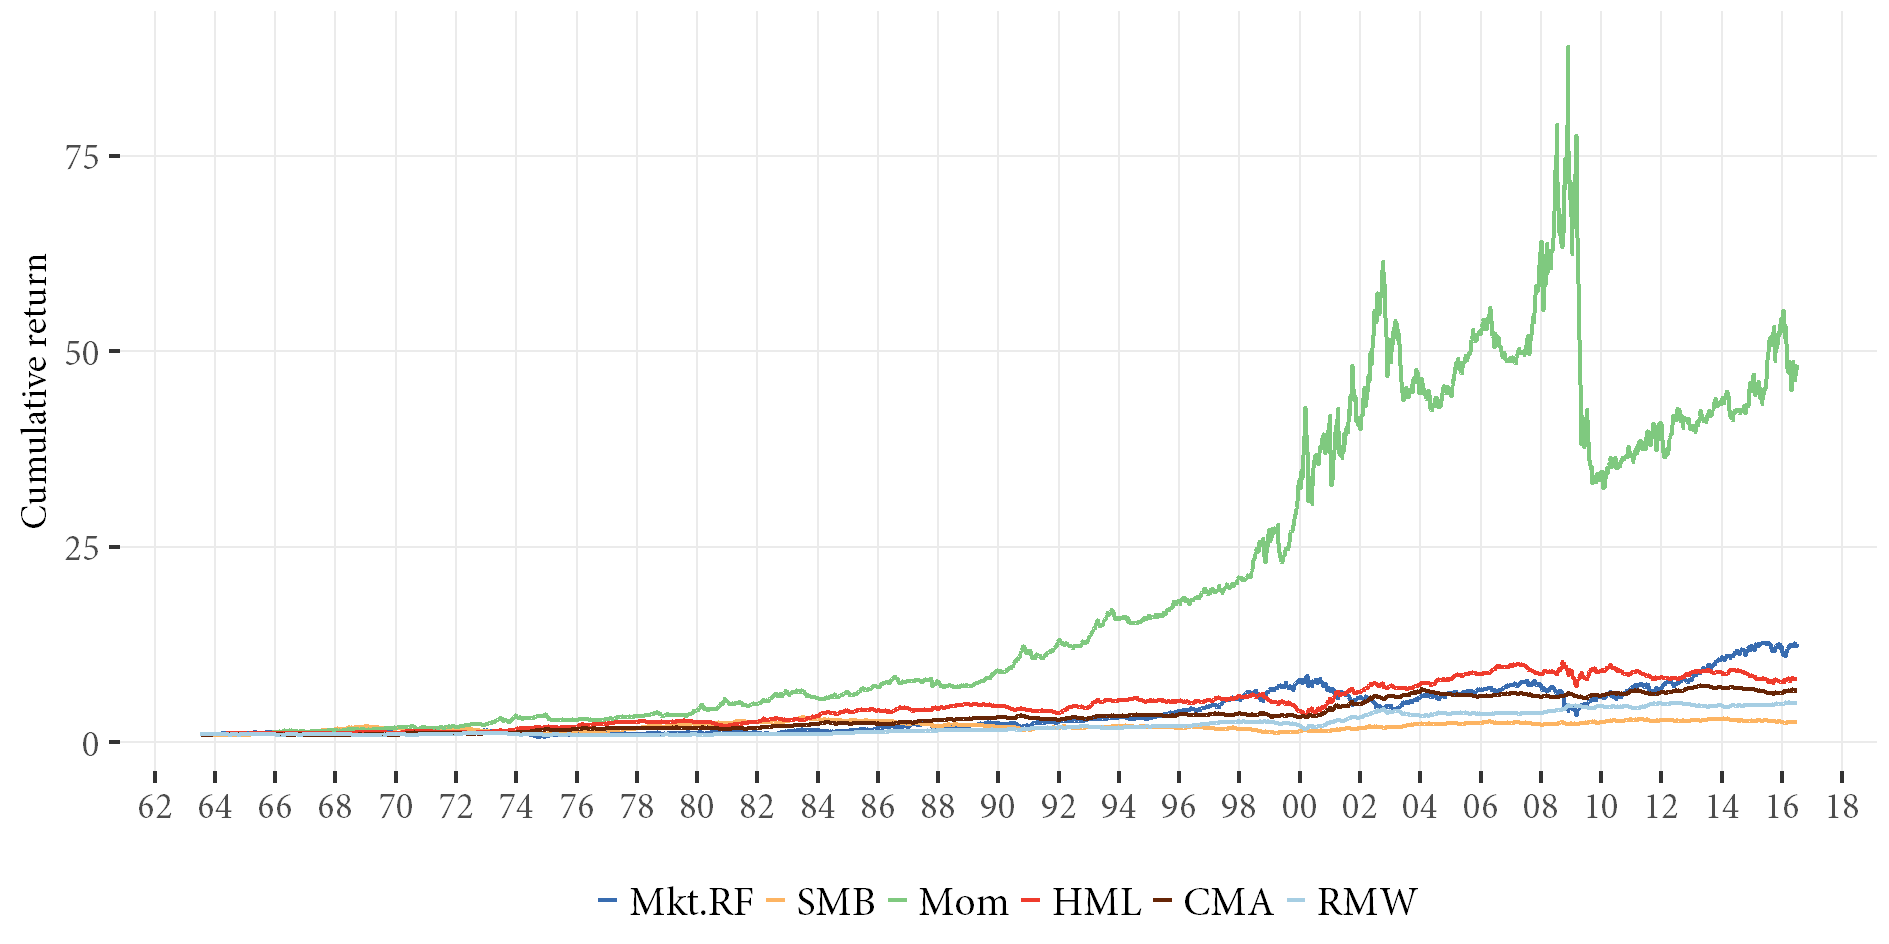
\includegraphics[scale=1]{graphics/cumretPlot.png}  
  %\bottomrule
  \vspace{3mm}
  \footnotesize
  Cumulative returns to investing one dollar in each factor strategy beginning 1963-07-05.  All data 1963-07-05 - 2016-07-01.
  \end{minipage}
\end{figure}
Plots of cumulative returns clearly show the high returns to the momentum strategy through the sample period. However, normalizing the series to 10\% annual volatility gives a more nuanced picture of mean-variance performance. Since 1963, each of the strategies except for SMB has outperformed the market factor. Furthermore, factor strategies seem to crash at different times and diversify eachother, e.g. Mom performing well during 1999-2000 and RMW performing well during 2008-2009.
\begin{figure}[H]
  \caption{Standardized cumulative returns to factor strategies}
  \label{diag:cumretstd}
  %\toprule
  \centering
  \begin{minipage}{\textwidth}
  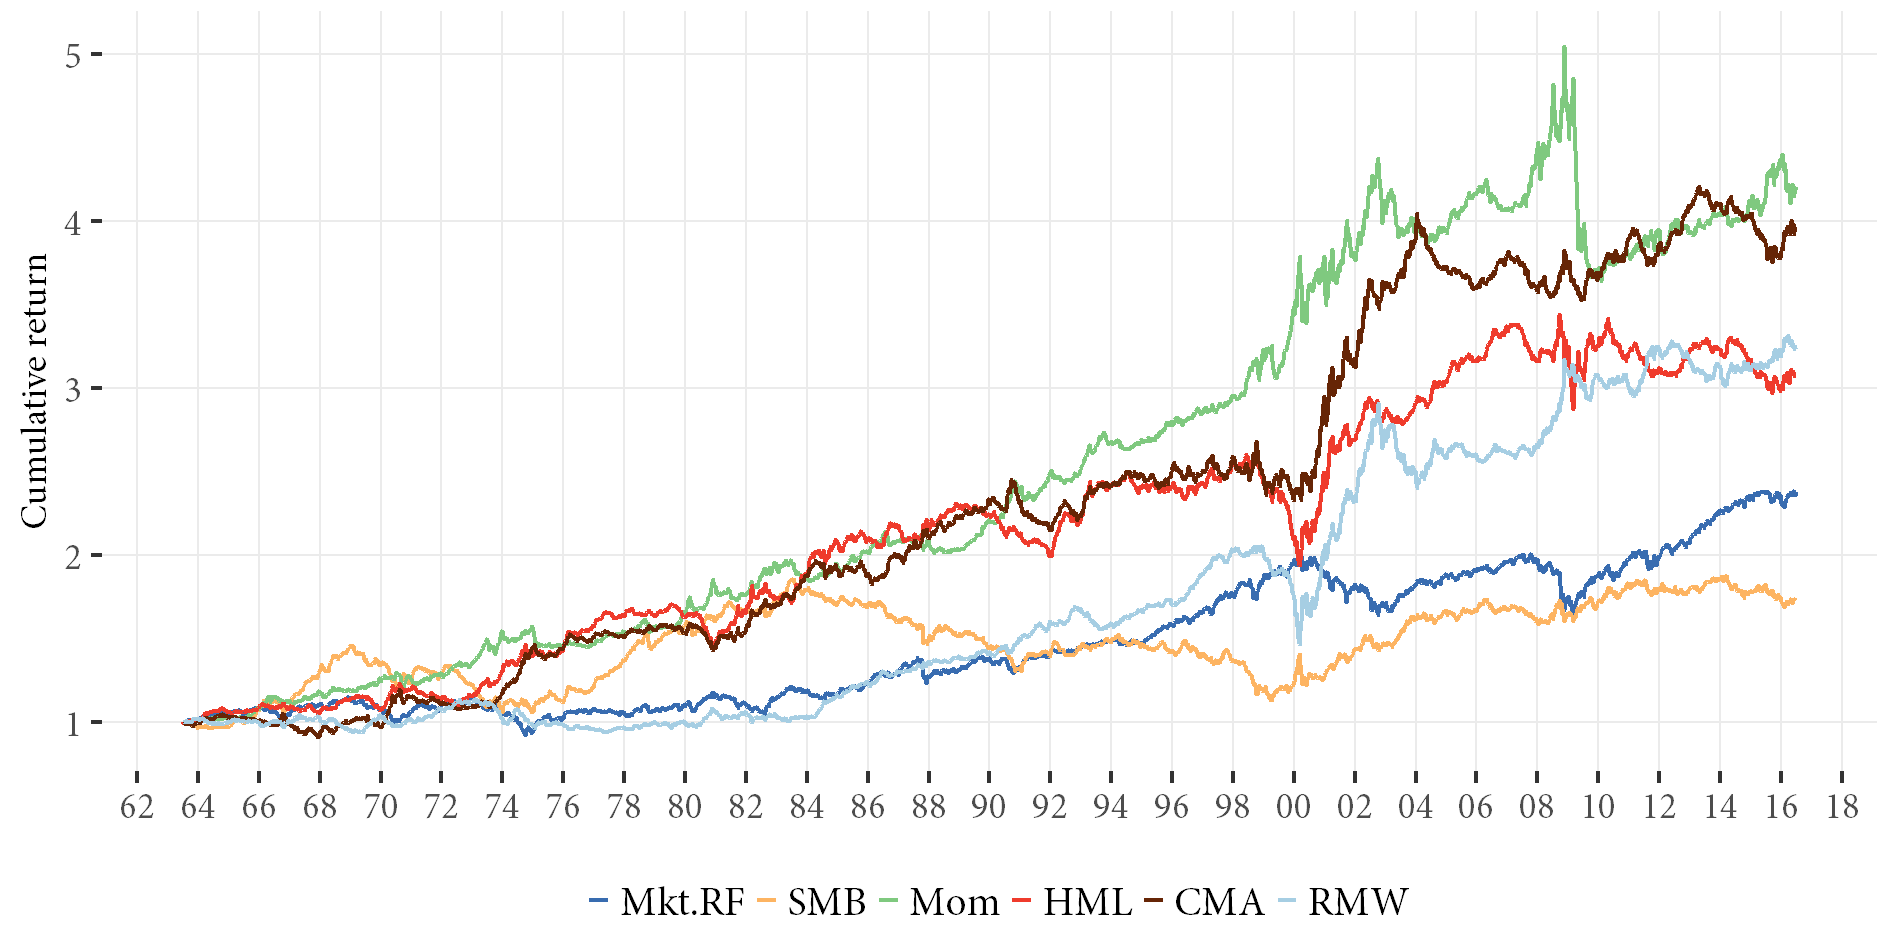
\includegraphics[scale=1]{graphics/cumretStdPlot.png}  
  %\bottomrule
  \vspace{3mm}
  \footnotesize
  Cumulative returns to investing one dollar in each factor strategy beginning 1963-07-05. Standardized to 10\% annual volatility. All data 1963-07-05 - 2016-07-01.
  \end{minipage}
\end{figure}
